\documentclass[nooutcomes,handout]{ximera}
\usepackage{fullpage}
\newcommand{\RR}{\mathbb R}
\renewcommand{\d}{\,d}
\newcommand{\dd}[2][]{\frac{d #1}{d #2}}
\renewcommand{\l}{\ell}
\newcommand{\ddx}{\frac{d}{dx}}
\newcommand{\dfn}{\textbf}
\newcommand{\eval}[1]{\bigg[ #1 \bigg]}

\usepackage{multicol}

\renewenvironment{freeResponse}{
\ifhandout\setbox0\vbox\bgroup\else
\begin{trivlist}\item[\hskip \labelsep\bfseries Solution:\hspace{2ex}]
\fi}
{\ifhandout\egroup\else
\end{trivlist}
\fi} 



\title{Briggs 5.3: Fundamental Theorem of Calculus}

\begin{document}
\begin{abstract}
\end{abstract}
\maketitle


%problem 1
\begin{problem}
  True of False: If $f$ is continuous on the closed interval $[a,b]$,
  then
  $$\ddx \left( \int_a^b f(t) \d t \right) = f(x)$$
  \begin{freeResponse}
    False.  $\ddx \left( \int_a^b f(t) \d t \right) = 0$
    since $\int_a^b f(t) \d t$ is a constant and
    $\ddx (\text{constant}) = 0$.
  \end{freeResponse}
\end{problem}

%problem 2
\begin{problem}
  The graph of $g$, a continuous function on $[0, 4]$, is shown in the figure.
  Let $A(x) = \int_{0}^x g(t) \d t$, for $0 \le x \le 4$.
  \begin{image}
    \includegraphics[scale = 0.4]{"Graph of function".png}
  \end{image}
  \begin{enumerate}
  
  	%part a
    \item
      Circle the correct statement about $A(2)$.
      \begin{enumerate}
        \item $A(2) = 0$;
        \item $A(2) > 0$;
        \item $A(2) < 0$;
        \item none of the previous answers.
      \end{enumerate}
      \begin{freeResponse}
        Correct choice: (iii) $A(2) < 0$.  The curve $g(t)$ on the interval $(0,2)$ is below the $x$-axis and therefore the net area is negative.
      \end{freeResponse}
      
      
	%part b
    \item
      Circle the correct statement about $A(3.8)$.
      \begin{enumerate}
        \item $A(3.8) = 0$;
        \item $A(3.8) > 0$;
        \item $A(3.8) < 0$;
        \item none of the previous answers.
      \end{enumerate}
      \begin{freeResponse}
        Correct choice: (ii) $A(3.8) > 0$.  The net area under the curve $g(t)$ on the interval $(2,3.8)$ is postive and larger than the negative net area on the interval $(0,2)$.  Therefore, the net area on the interval $(0,3.8)$ is positive.
      \end{freeResponse}

	%part c
    \item
      Circle the correct statement about $A'(3.8)$.
      \begin{enumerate}
        \item $A'(3.8) = 0$;
        \item $A'(3.8) > 0$;
        \item $A'(3.8) < 0$;
        \item none of the previous answers.
      \end{enumerate}
      \begin{freeResponse}
        Correct choice: (ii) $A'(3.8) > 0$ because $A'(3.8)=g(3.8)$
      \end{freeResponse}

	%part d
    \item
      Find the solution of the following initiual value problem: $y'(x) = g(x)$ and $y(0) = 2$.
      \begin{enumerate}
        \item $y(x) = g(x)$;
        \item $y(x) = g(x) + 2$;
        \item $y(x) = A(x)$;
        \item $y(x) = A(x) + 2$;
        \item $y(x) = g'(x)$;
        \item $y(x) = g'(x) + 2$;
        \item none of the previous answers.
      \end{enumerate}
      \begin{freeResponse}
        Correct choice: (iv) $y(x) = A(x) + 2$.  $y'(x)=A'(x)=g(x)$ and $y(0)=A(0)+2=2$
      \end{freeResponse}

	%part e
    \item
      Find the expression for $\int_0^4 |g(t)| \d t$.
      \begin{enumerate}
        \item $A(4)$;
        \item $A(2) - A(4)$;
        \item $A(4) - A(2)$;
        \item $A(4) - 2 A(2)$;
        \item none of the previous answers.
      \end{enumerate}
      \begin{freeResponse}
        Correct choice: (iv) $A(4) - 2 A(2)$.  \\
        $$\int_0^4 |g(t)| \d t = \int_2^4 g(t) \d t-\int_0^2 g(t) \d t  $$
       and  $$\int_2^4 g(t) \d t =\int_0^4 g(t) \d t-\int_0^2 g(t) \d t $$
       Therefore, $$\int_0^4 |g(t)| \d t = \int_0^4 g(t) \d t-2\int_0^2 g(t) \d t =A(4)-2A(2) $$
      \end{freeResponse}

	%part f
    \item
      Find the midpoint Riemann sum for the function $g$ on the interval $[0, 4]$ with $n = 2$ (the number of subintervals).
      \begin{enumerate}
        \item $g(1) + g(3)$;
        \item $g(0) + g(2)$;
        \item $g(2) + g(4)$;
        \item $2g(1) + 2g(3)$;
        \item $2g(0) + 2g(2)$;
        \item $2g(2) + 2g(4)$;
        \item none of the previous answers.
      \end{enumerate}
      \begin{freeResponse}
        Correct choice: (iv) $2g(1) + 2g(3)$
        
        \begin{image}
        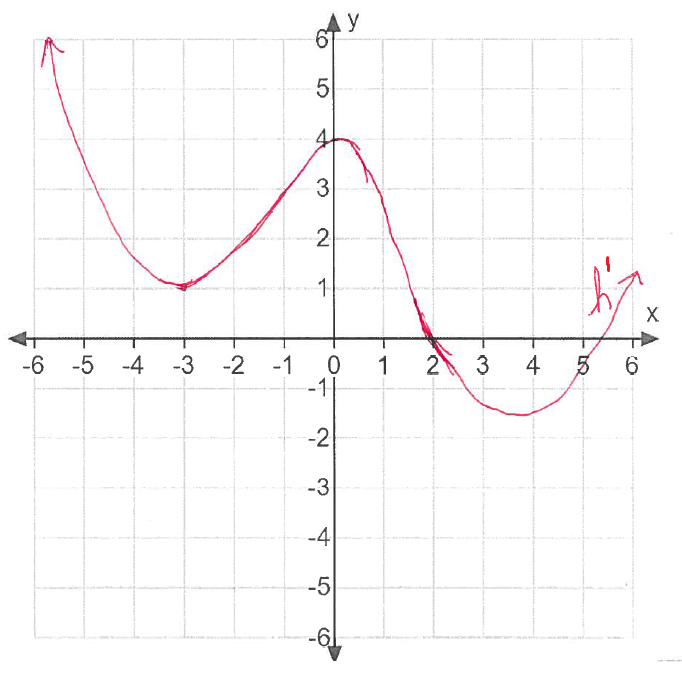
\includegraphics[scale=.6]{figure1.png}
        \end{image}
      \end{freeResponse}
  \end{enumerate}


\end{problem}

%problem 3
\begin{problem}
  The \underline{limit of Riemann sums} for a function $f$ on the interval $[1, 5]$ is given by
  \[
    \lim_{\Delta \to 0} \sum_{k = 1}^n \left(2x_k^* + \frac{1}{x_k^*} \right) \Delta x_k\mbox{ on $[1, 5]$.}
  \]
  \begin{enumerate}
    \item
      Identify $f$ and express the limit as a \underline{definite integral}.
      \begin{freeResponse}
       
        $$f(x)=2x+\frac{1}{x}$$\\
        $$\int_1^5 \left( 2x + \frac{1}{x} \right) \d x = \lim_{\Delta \to 0} \sum_{k = 1}^n \left(2x_k^* + \frac{1}{x_k^*} \right) \Delta x_k$$
      
      \end{freeResponse}

    \item
    Evaluate the \underline{limit of Riemann sums}.
    \begin{freeResponse}
      \[
        \int_1^5 \left( 2x + \frac{1}{x} \right) \d x = \left(x^2 + \ln|x|\right) \bigm|_1^5 = (25 + \ln(5)) - (1 +\ln(1)) = 24 +\ln(5)
      \]
    \end{freeResponse}
  \end{enumerate}
  
\end{problem}

%problem 4
\begin{problem}
  Compute the following integrals:
  \begin{enumerate}
    

  \item  $\int_0^1 e^{5x} \d x$
    \begin{freeResponse}
      $\int_0^1 e^{5x} \d x  = \eval{\frac{1}{5} e^{5x}}_0^1= \frac{1}{5} \left( e^5 - e^0 \right) = \frac{1}{5} (e^5 - 1)$
    \end{freeResponse}
    

  \item  $\int\limits_{-2}^{-1} \frac{1}{x^3} \d x$
    \begin{freeResponse}
      \begin{align*}
        \int\limits_{-2}^{-1} \frac{1}{x^3} \d x &= \int\limits_{-2}^{-1} x^{-3} \d x  \\
                                                 &= \eval{\frac{x^{-2}}{-2}}_{-2}^{-1}  \\
                                                 &= \eval{\frac{-1}{2x^2}}_{-2}^{-1}  \\
                                                 &= - \frac{1}{2} - \left( - \frac{1}{8} \right)  \\
                                                 &= - \frac{1}{2} + \frac{1}{8} = - \frac{3}{8}
      \end{align*}
    \end{freeResponse}

  \item  $\int _0^4 \left( 3x - 5 + 7 \sqrt{16-x^2} \right) \d x$
    \begin{freeResponse}
      First notice that:
      \begin{equation}\label{eq1}
        \int _0^4 \left( 3x - 5 + 7 \sqrt{16-x^2} \right) \d x = \int_0^4 ( 3x - 5) \d x + 7 \int_0^4 \sqrt{16-x^2} \d x.
      \end{equation}
      To get the easy part out of the way first:
      \begin{equation}\label{eq2}
        \int_0^4 (3x-5) \d x = \eval{\frac{3}{2} x^2 - 5x}_0^4 = (24 - 20) - (0-0) = 4. 
      \end{equation}
      So the real issue is in computing $\int_0^4 \sqrt{16-x^2} \d x$.  
      
      We do not know how to integrate $\sqrt{16-x^2}$ directly, but recall that the solution set to the equation $x^2 + y^2 = 16$ is a circle with radius $4$ centered at the origin.  
      Solving for $y$ we get $y = \pm \sqrt{16-x^2}$.  
      So if we restrict ourselves to $y=\sqrt{16-x^2}$ and $0 \leq x \leq 4$, this gives us the upper-right quarter of the circle (draw a picture and convince yourself of this).  
      Since the total area of the circle of $\pi (4)^2 = 16\pi$, the area under this portion of the curve is $\frac{1}{4} (16\pi) = 4\pi$.  
      Thus we have computed (geometrically) that 
      \begin{equation}\label{eq3}
        \int_0^4 \sqrt{16-x^2} \d x = 4\pi. 
      \end{equation}
      So, $\int _0^4 \left( 3x - 5 + 7 \sqrt{16-x^2} \right) \d x = 4 + 7(4\pi) = 4 + 28\pi$ by (1),(2), and (3)
      \end{freeResponse}
  \end{enumerate}
\end{problem}

%problem 5
\begin{problem}
  Find the derivative of the following functions:
  \begin{enumerate}
    
%part a
  \item  $F(x) = \int_{\sqrt{x}}^1 \frac{t^2}{2 + 3t^4} \d t$
    \begin{freeResponse}
      First notice that
      $$ F(x) = \int_{\sqrt{x}}^1 \frac{t^2}{2 + 3t^4} \d t = - \int^{\sqrt{x}}_1 \frac{t^2}{2 + 3t^4} \d t .$$
      So we can apply the Fundamental Theorem of Calculus Part I, along with the chain rule, to compute:
      \begin{align*}
        F^\prime (x) &= \ddx \left( - \int^{\sqrt{x}}_1 \frac{t^2}{2 + 3t^4} \d t \right)  \\
       \text{we introduce the variable:}\ u=\sqrt x \implies F'(x)&=\frac{dF}{du}\frac{du}{dx}\\ 
                     &= - \frac{u^2}{2 + 3(u)^4} \cdot \ddx(\sqrt{x})  \\
                     &= - \frac{u^2}{2+3u^4} \cdot \frac{1}{2 \sqrt{x}}  \\
            \text{substituting}\ u=\sqrt x \implies          F^\prime (x) &= - \frac{x}{2+3x^2} \cdot \frac{1}{2 \sqrt{x}}  \\
            		&= - \frac{\sqrt{x}}{2(2+3x^2)}  
      \end{align*}
    \end{freeResponse}
    
    
    %part b
  \item  $G(x) = \int_x^{x^3} \sin(7t) \d t$
    \begin{freeResponse}
      First notice that
      \begin{align*}
        G(x) &= \int_x^{x^3} \sin(7t) \d t  \\
             &= \int_x^0 \sin(7t) \d t + \int_0^{x^3} \sin(7t) \d t  \\
             &=  - \int^x_0 \sin(7t) \d t + \int_0^{x^3} \sin(7t) \d t
      \end{align*}
      It is worth pointing out that breaking up the integral above at $0$ was arbitrary.  Since $\sin(7t)$ is continuous over $(-\infty, \infty)$, we could have chosen any real number in place of $0$.
      
      We can now apply the Fundamental Theorem of Calculus Part I, along with the chain rule, to compute:
      \begin{align*}
        G^\prime (x) &= \ddx \left( - \int^x_0 \sin(7t) \d t + \int_0^{x^3} \sin(7t) \d t \right)  \\
                     &= \ddx \left( - \int^x_0 \sin(7t) \d t \right) + \ddx \left( \int_0^{x^3} \sin(7t) \d t \right)  
        \end{align*}
        The left integral requires no chain rule on the FTC Part I.  $ \ddx \left( - \int^x_0 \sin(7t) \d t \right)=-\sin(7x)\\$
        
        The right integral requires chain rule.  We'll subsitute $u=x^3$.
        \begin{align*}
       \ddx \left( \int_0^{x^3} \sin(7t) \d t \right) &= \dd{u} \left( \int_0^{u} \sin(7t) \d t \right) \dd[u]{x}\\
                                 &=\sin(7u) \cdot \ddx(x^3)\\
                                 &=\sin(7u) \cdot 3x^2\\
 	\text{substituting}\ u=x^3  \implies \ddx \left( \int_0^{x^3} \sin(7t) \d t \right) &=3x^2 \sin(7x^3)
           \end{align*}
           Combining we have: 
                  $$G^\prime (x) = 3x^2 \sin(7x^3) - \sin(7x)$$
  
    \end{freeResponse}
  \end{enumerate}
\end{problem}

%problem 6
\begin{problem}
  Given the following graph of $y=f(x)$, let $g(x) = \int_{-1}^x f(t) \d t$.
  
      \begin{image}
      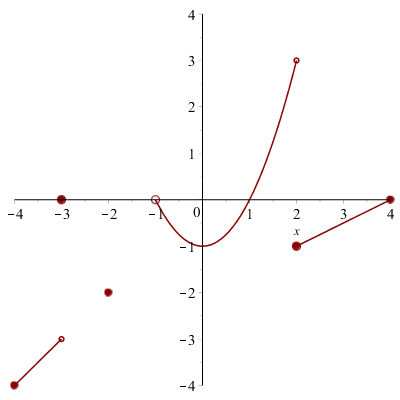
\includegraphics{Figure2.png}
    \end{image}
  
  \begin{enumerate}

  \item  Is $g$ continuous?  Why or why not?
     \begin{freeResponse}
     $g(x)$ represents the area function (or the signed area between the curve $y=f(x)$ and the $x$-axis from -1 to $x$).  By the FTC(I), $g(x)$ is continuous.
    \end{freeResponse}
    
    
    
    % part b
  \item  Is $g$ differentiable?  Why or why not?
     \begin{freeResponse}
    Similarly by the FTC(I) the function $g$ is differentiable, and moreover:
        $$\ddx \left( g(x) \right) = \ddx \left( \int_{-1}^x f(t) \d t \right)= f(x)$$
     \end{freeResponse}
    
    
    
    % part c
  \item  Where does $g$ achieve its absolute maximum and minimum values?  Where does $g$ achieve any local extreme values?  Assume the domain of $g$ is $[-1,7.6]$.
    \begin{freeResponse}
    Since $g$ is continuous on the closed interval $[-1,7.6]$, $g$ attains its absolute extreme values at either critical points or endpoints.  
        But we just saw that $g^\prime(x) = f(x)$, and so the critical points of $g$ are just the points where $f(x) = 0$.  
        Thus, the critical points of $g$ are approximately $3.1$ and $6.25$.
        
        Since $f = g^\prime$, $g$ is increasing when $f$ is positive and $g$ is decreasing when $f$ is negative.  
        So we have that $x=3.1$ is a local maximum while $x=6.25$ is a local minimum of $g$.  
        This takes care of the local extreme values.  
        
        To find the absolute extreme values of $g$, we need to determine what are the largest and smallest values among $g(-1), g(3.1), g(6.25),$ and $g(7.6)$.  
        And do not forget the $g(x)$ denotes the (signed) area of the region bounded by the curve and the $x-axis$.
        
        Clearly $g(-1) = 0$ since a line segment does not have any area.  
        At any time after $x=-1$ we have a positive (net) area.  
        Thus, our absolute minimum occurs at $x=-1$.
        To find the absolute maximum of $g$, we need to compare $g(3.1)$ and $g(7.6)$. 
        We see that we have the greatest area under the curve at $x=3.1$ because 
        by the time we get to $x=7.6$, the area we have subtracted off between $x=3.1$ and $x=6.25$ is greater than 
        what we have added back on from $x=6.25$ to $x=7.6$.  
        Therefore, our absolute maximum occurs at $x=3.1$.  
     \end{freeResponse}
    
    
    
    % part d
  \item  Where is the graph of $g$ concave up?  Concave down?
    \begin{freeResponse}
     $g$ is concave up when when $f$ is increasing, which is on $(-1,0) \cup (4.25,7.6)$.  
        Similarly, $g$ is concave down when $f$ is decreasing, which is on $(0,4.25)$.  Remember, $g'=f$.
    \end{freeResponse}


  \end{enumerate}
\end{problem}


%problem 7
\begin{problem}
  The graph of $g$, a continuous function $[0, 4]$, is shown in the figure.
  Let $A(x) = \int_0^x g(t) \d t$ for $0 \le x \le 4$.
  \begin{image}
    \includegraphics[scale = 0.4]{"Graph of continuous function".png}
  \end{image}
  \begin{enumerate}
  
  	%part a
    \item
      Circle the correct statement about $A(1)$.
      \begin{enumerate}
        \item $A(1) = 0$;
        \item $A(1) < 0$;
        \item $A(1) > 0$;
        \item none of the previous answers.
      \end{enumerate}
      \begin{freeResponse}
        Correct choice: (ii) $A(1) < 0$.  $A(1)$ is the net area of the region bounded by the curve and the $x$-axis between $x=0$ and $x=1$.  On this interval, $g(t)$ is negative and therefore, $ A(1)$ is negative.
      \end{freeResponse}

%part b
    \item
      Circle the correct statement about $A(1.5)$.
      \begin{enumerate}
        \item $A(1.5) = 0$;
        \item $A(1.5) < 0$;
        \item $A(1.5) > 0$;
        \item  none of the previous answers.
      \end{enumerate}
      \begin{freeResponse}
        Correct choice: (ii) $A(1.5) < 0$  The net area on the interval $(1,1.5)$ is postive and smaller than the negative net area on the interval $(0,1)$.  Therefore, the net area on the interval $(0,1.5)$ is negative.
      \end{freeResponse}

%part c
    \item
      Circle the correct statement about $A'(1.5)$.
      \begin{enumerate}
        \item $A'(1.5) = 0$;
        \item $A'(1.5) < 0$;
        \item $A'(1.5) > 0$;
        \item none of the previous answers.
      \end{enumerate}
      \begin{freeResponse}
        Correct choice: (iii) $A'(1.5) > 0$  because $A'(1.5)=g(1.5)$
      \end{freeResponse}

%part d
    \item
      Circle the correct expression for $\int_1^4 (g(t) + 1) \d t$.
      \begin{enumerate}
        \item $A(4) + 1$;
        \item $A(4) - A(1)$;
        \item $A(4) - A(1) + 1$;
        \item $A(4) + 3$;
        \item $A(4) - A(1) + 3$;
        \item none of the previous answers.
      \end{enumerate}
      \begin{freeResponse}
        Correct choice: (v) $A(4) - A(1) + 3$
        
        	We can split the integral: $\int_1^4 (g(t) + 1) \d t = \int_1^4 g(t) \d t +\int_1^4  1 \d t =A(4)-A(1)+3$ 
        
        We can visualize this integal by imagining shifting the graph of $g$ up one unit. See figure below.  Our area we are looking for consists of the area under the curve $g$ on the interval $(1,4)$ (the blue region) plus the rectangular region formed below (the purple region).\\
        

            
              \begin{image}
    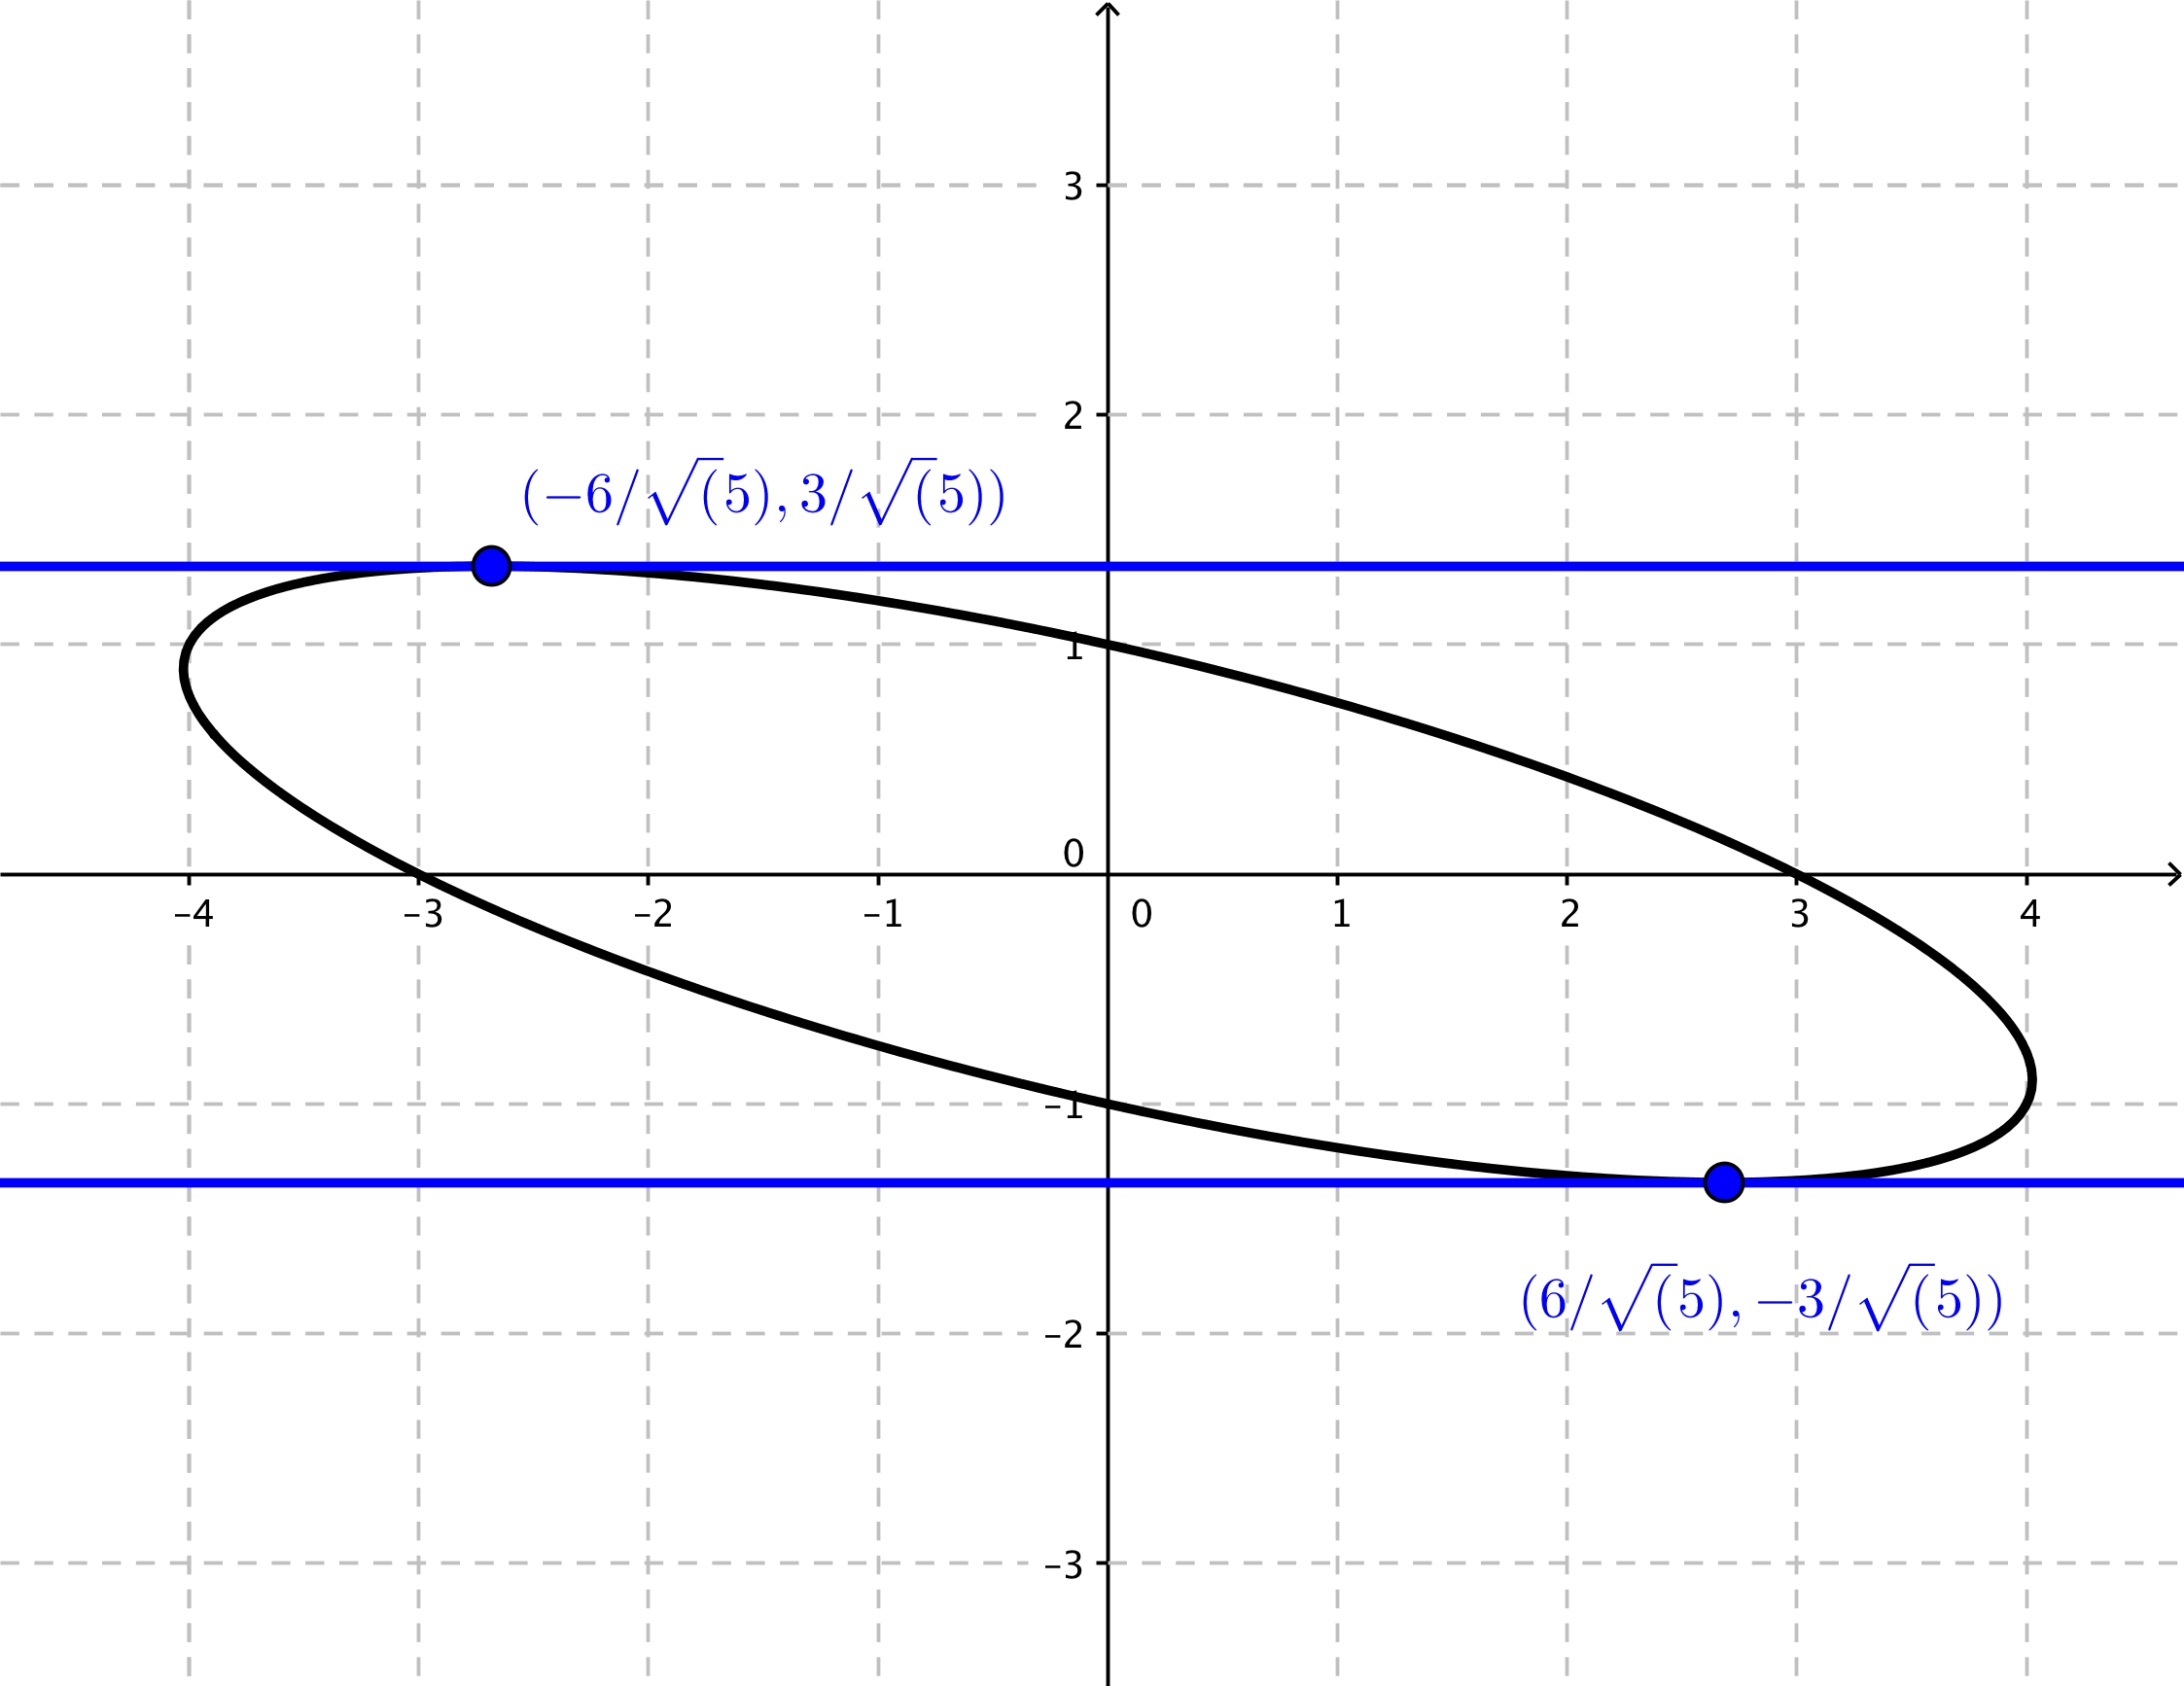
\includegraphics[scale = 0.5]{figure3.png}
  \end{image}
            
            The area of the blue region is  $\int_1^4 g(t) \d t= \int_0^4 g(t) \d t- \int_0^1 g(t) \d t=A(4)-A(1)$.
            
            The area of the purple region is $\int_1^4  1 \d t$.  This integral is the area under the line $y=1$ on the interval $(1,4)$ which is a rectangular region of area $3$.
            
             Combining these, the total area  $\int_1^4 (g(t) + 1) \d t = A(4)-A(1)+3$
            
            
            
      \end{freeResponse}

% part e
    \item
      Circle the correct statement about $A(0)$.
      \begin{enumerate}
        \item $A(0) = 0$;
        \item $A(0) = 1$;
        \item $0 < A(0) < 1$;
        \item $A(0) > 1$;
        \item $A(0) < 0$;
        \item none of the previous answers.
      \end{enumerate}
      \begin{freeResponse}
        Correct choice: (i) $A(0) = 0$.  By the definition of $A$, $A(x)=\int_0^x g(t) \d t$ for $0 \le x \le 4$. So, $A(0)=\int_0^0 g(t) \d t=0$.  
      \end{freeResponse}

% part f
    \item
      Circle the interval (or intervals) where the function $A$ is DECREASING.
      \begin{enumerate}
        \item $(0, 1)$;
        \item $(1, 2)$;
        \item $(2, 4)$;
        \item none of the previous answers.
      \end{enumerate}
      \begin{freeResponse}
        Correct choice: (i) $(0, 1)$.  $A$ is decreasing means that the area is decreasing or we are accumulating negative area.  This happens when $A$'s derivative, $g$ is negative.
      \end{freeResponse}

%part g
    \item
      Circle the value (or values) where the function $A$ attains its MAXIMUM.
      \begin{enumerate}
        \item $x = 0$;
        \item $x = 1$;
        \item $x = 2$;
        \item $x = 3$;
        \item $x = 4$;
        \item none of the previous answers.
      \end{enumerate}
      \begin{freeResponse}
        Correct choice: (v) $x = 4$.  It appears that $A(x)<0$ on $(0,2)$ and $A(x)>0$ on $(2,4]$.  So, the maximum occurs on $[2,4]$.  Since $A'=g$ is postive on $(2,4)$, and $A$ is increasing there, the maximum is attained at the end point, $x=4$.  In other words, $A$ achieves a maximum when we have the largest potive area.  Because we start with negative area and then continue to accumulate positive area until $x=4$, the maximum occurs at the end point.
      \end{freeResponse}

%part h
    \item
      Circle the value  (or values) where the function $A$ attains its MINIMUM.
      \begin{enumerate}
        \item $x = 0$;
        \item $x = 1$;
        \item $x = 2$;
        \item $x = 3$;
        \item $x = 4$;
        \item none of the previous answers.
      \end{enumerate}
      \begin{freeResponse}
        Correct choice: (ii) $x = 1$.  $A'=g$ is negative on $(0,1)$ and positive on $(1,4)$.  So $A$ is decreasing on $(0,1)$ and increasing on $(1,4)$.  So the local and absolute maximum occurs at $x=1$.  In other words, $A$ achieves a minimum when we have the largest negative area.  We start by accumulating negative area and then switch to accumulating positive area at $x=1$.
      \end{freeResponse}

%item i
    \item
      Circle the interval (or intervals) where the function $A$ is CONCAVE DOWN.
      \begin{enumerate}
        \item $(0, 1)$;
        \item $(1, 2)$;
        \item $(2, 4)$;
        \item none of the previous answers.
      \end{enumerate}
      \begin{freeResponse}
        Correct choice: (iii) $(2, 4)$.  $A$ is concave down where $A'=g$ is decreasing.  $g$ is decreasing on $(2,4)$. 
      \end{freeResponse}

  \item
      Circle the value (or values) of $x$ where the function $A$ has an inflection point.
      \begin{enumerate}
        \item $x = 1$;
        \item $x = 2$;
        \item $x = 3$;
        \item none of the previous answers.
      \end{enumerate}
      \begin{freeResponse}
        Correct choice: (ii) $x=2$.  $A'=g$ changes from increasing to decreasing.
      \end{freeResponse}

  
  \item Sketch the graph of $A$, based on items (e)-(j)
  
        \begin{freeResponse} \hfil
                      \begin{image}
    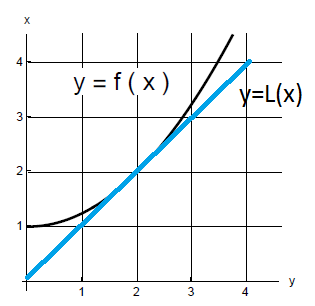
\includegraphics[scale = 0.7]{figure4.png}
  \end{image}
      \end{freeResponse}
  
    \end{enumerate}
\end{problem}
\end{document} 
